\subsection*{3.1 - 3.3} 
Per definition, we assume that a negative capacity allows flow to be
directed backwards through an edge. This means the edge (v,w) with upper
capacity u and lower capacity l, can be treated as an anti-par of edges.
With both edges (v,w),(w,v) having the lower capacity 0 and upper capacity
u and l respectively.
\begin{figure}[!ht]
    \resizebox{\columnwidth}{!}{
        \centering
        \begin{subfigure}[b]{0.40\textwidth}
            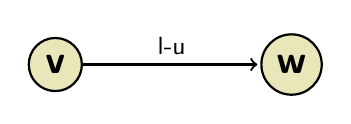
\begin{tikzpicture}[->,shorten >=1pt,auto,node distance=3cm,
  thick,main node/.style={circle,fill=olive!20,draw,font=\sffamily\Large\bfseries}]

  \node[main node] (1) {v};
  \node[main node] (2) [right of=1] {w};
  \coordinate[above of=2] (d1); 

  \path[every node/.style={font=\sffamily\small}]
  (1)  edge [] node[above] {l-u} (2);
\end{tikzpicture}

        \end{subfigure}
        \begin{subfigure}[b]{0.40\textwidth}
            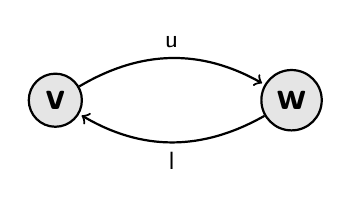
\begin{tikzpicture}[->,shorten >=1pt,auto,node distance=3cm,
  thick,main node/.style={circle,fill=gray!20,draw,font=\sffamily\Large\bfseries}]

  \node[main node] (1) {v};
  \node[main node] (2) [right of=1] {w};

  \path[every node/.style={font=\sffamily\small}]
  (1)  edge [bend left] node[above] {u} (2)
  (2)  edge [bend left] node[below] {l} (1);
\end{tikzpicture}

        \end{subfigure}
        \begin{subfigure}[b]{0.40\textwidth}
            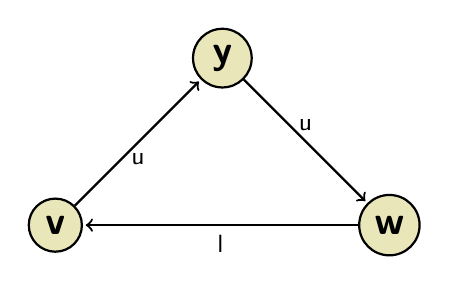
\begin{tikzpicture}[->,shorten >=1pt,auto,node distance=3cm,
  thick,main node/.style={circle,fill=olive!20,draw,font=\sffamily\Large\bfseries}]

  \node[main node] (1) {y};
  \node[main node] (2) [below right of=1] {w};
  \node[main node] (3) [below left of=1] {v};

  \path[every node/.style={font=\sffamily\small}]
     (1)  edge [] node[above] {u} (2)
     (2)  edge [] node[below] {l} (3)
     (3)  edge [] node[below] {u} (1);
\end{tikzpicture}

        \end{subfigure}
    }
    \caption{the transformation to be done on each edge (v,w)}
    \label{fig:anti-transform}
\end{figure}
We will now show the transforming $I_0$ to $I_1$ as shown on Figure \ref{fig:anti-transform} leaves a flow with $l_e = 0$ for each edge.

We assume $I_0$ is a flow satisfying flow conservation and the modified capacity constraint (\ref{con:cap}).
\begin{equation} \label{con:cap}
    \text{For all } u, v \in V \text{, we require }l(u,v) \le f(u,v) \le c(u,v)
\end{equation}

The modified network still obeys flow conservation. As the flow from v to
w is changed from negative x to 0 while the incoming flow from w through y
is x. Leaving the note at negative x flow. 

The change also obeys the capacity constraint. Before the modification the
vertex obeys the modified capacity constraint. Removing the negative value
edge from v increases the lower bound of the node capacity to 0, but since
it does not modify positive edges of the upper bound, all other outgoing
edges should still uphold the constraint.\\ 
This solves the first 3 subexercises of exercise 3.
